\documentclass{article}

\usepackage{todonotes}
\usepackage[colorlinks=true]{hyperref}
\usepackage[framed,numbered,autolinebreaks]{mcode}
\usepackage{fullpage}
\usepackage{url,textcomp}
\setlength{\parindent}{0pt}
\setlength{\parskip}{18pt}
\title{MATLAB Introduction}
\author{Rob Campbell \& Maxime Rio}
\date{}
% //////////////////////////////////////////////////

\renewcommand{\familydefault}{\sfdefault}
\usepackage{helvet}
\usepackage[compact]{titlesec}
\usepackage{microtype}
\titlespacing\subsection{0pt}{12pt plus 4pt minus 2pt}{0pt plus 0pt minus 5pt}

\usepackage{enumitem} %easily change item spacing
\setitemize{noitemsep} % sets no itemsep for enumerate lists only

\begin{document}

\maketitle


\section*{Introduction}

MATLAB is a fairly simple programming language designed to make analysis of data easy.
It is commonly used in academic research, industry, and finance.
Today you will learn the basics of MATLAB.
Once you have mastered this, on the remaining three days you will get to do more exciting stuff such as analyze real 2-photon imaging data from mice, acquire your own action potential data with electrodes, and then analyse these data.


\subsection*{What you will learn today}
\begin{itemize}
\item That MATLAB stores data in \textbf{variables}.
\item How MATLAB variables store lists of numbers and text (`strings').
\item How variables are manipulated by \textbf{functions}. e.g. to perform mathematical operations and plot data.
\item Chaining functions together using \textbf{loops} and \textbf{logic statements} to automate sequences of operations.
\end{itemize}

An important aspect of today's practical is that you learn how to use MATLAB's help and documentation.
Pay attention where we ask you read help and documentation pages. Ask us if the documentation does not make sense to you.
If you get stuck, first try to look up your problem using MATLAB's documentation or Google.
If you continue to be stuck, ask for help.
\textbf{\emph{You will not be able to complete subsequent practical sessions if you have not understood} all \emph{the concepts covered today}}.
If you are confused: ask for assistance.

\pagebreak
\section{Starting MATLAB}
On Linux machines, use \emph{Applications/Education/Matlab} menu entry to start MATLAB.
You should see an interface similar to Figure~\ref{fig:interface}.
Take two minutes to identify the two major components you will deal with:
\begin{itemize}
\item the \textbf{command line}, which you'll use to interact with MATLAB,
\item the \textbf{workspace} panel, where you'll keep track of manipulated data (`variables').
\end{itemize}

Finally, note the \textbf{New Script} button, that will be useful to create new \textbf{function} files,
and the \textbf{change directory} button to change the current directory you will be working in. MATLAB will
look for the functions you write in the current directory.

\begin{figure}[h]
  \centering
  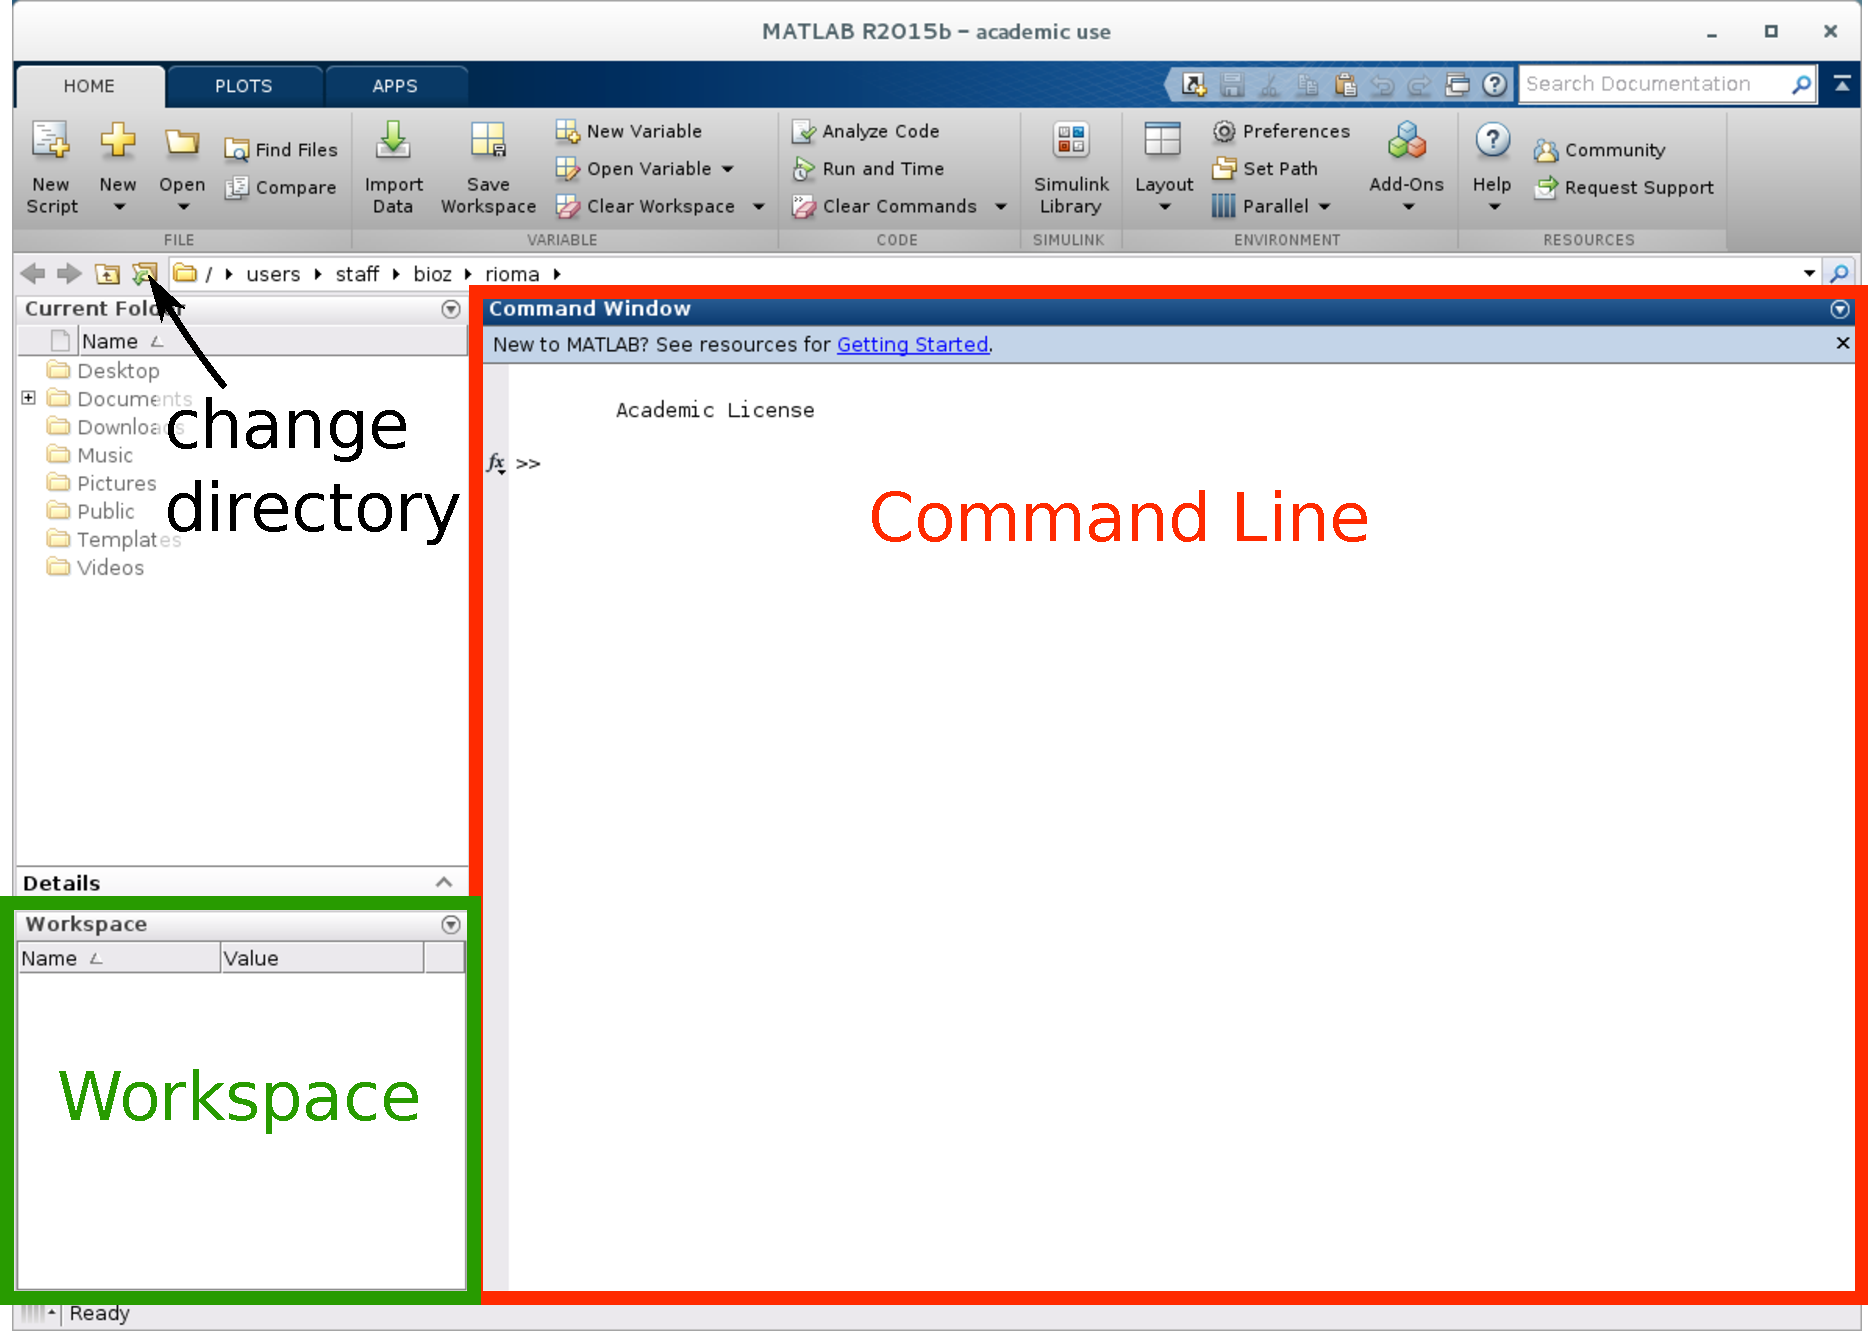
\includegraphics[width=0.7\textwidth]{interface.pdf}
  \caption{MATLAB interface major components}\label{fig:interface}
\end{figure}

\pagebreak

\subsection*{Experience the power of MATLAB: the command line}
Throughout today you will be typing stuff in to the \textbf{command line}, where you see the \verb|>>| symbol.
We will be asking you to type commands in the space after the \verb|>>| symbol.
To get you started, let's see the power of MATLAB using a few lines of code.
Type the following \emph{exactly} as shown into the command line and press return after each line.\\

\begin{itemize}
\item Get MATLAB to download an image from the internet using the \mcode{webread} \textbf{function}:\\
\verb|im=webread('http://mouse.vision/pic.jpg');|\\
\item Get MATLAB to show this image (WARNING: image isn't pretty):\\
\verb|imshow(im)|\\
\item Let's attempt to increase the elegance of the image. Black and white should help:\\
\verb|imshow( im(:,:,2) )|\\
\item That didn't help very much. Let's get rid this horrible image:\\
\verb|close all|\\
\item That's better. Lets also get rid of the \textbf{variable}, \mcode{im}, that produced it:\\
\verb|clear im|\\
\end{itemize}

Good stuff: that was your first experience of the power of MATLAB.
As you can see, it's  scary stuff: you downloaded an image, displayed it, modified it, then got rid of it.
But what exactly do all those commands do?
By the end of today you will have learned enough to easily understand what was going on in the above code.
Let's dive in\ldots

\pagebreak
\section{Calculations in MATLAB}

We will begin by treating MATLAB as a graphical calculator.
This is less interesting than what you just did, but we have to cover the basics first.

\verb|>>| \mcode{1} \\
then press return. \\
See how it echoes the number back to you? Now type: \\
\verb|>>| \mcode{1;} \\
Note the presence of the \mcode{;} (semicolon) symbol.
See how it no longer echoes the number back to you?
The \mcode{;} suppresses the echo.
You will use this feature a lot so keep it in mind.

Numbers are not limited to positive integers.
You can also enter real numbers, for example \\
\verb|>> 0.012| \\
or with a scientific notation \\
\verb|>> 1.2e-2| \\
and negative values, using a \mcode{-} (minus) sign:\\
\verb|>> -3.5| \\

Now let's look at basic arithmetic operators.
Type the following into the command line.
We leave off the semicolon so you can see the output.
The small numbers to the left are just line number labels, do not type them into the command line.

\begin{lstlisting}
4 + 10
4 - 10
4 * 10
4 / 10
4^3
\end{lstlisting}
What does the last line (\mcode{4^3}) do?

Of course you can use several operators on the same line, but be careful with their priority.
You can force the order of the operations using parentheses.
Compare the results from the following lines:
\begin{lstlisting}
4 + 2 * 3 - 1
(4 + 2) * 3 - 1
(4 + 2) * (3 - 1)
\end{lstlisting}

To conclude this first part, enter the following into the command line: \\
\verb|>>| \mcode{\%This is a comment.} \\
After pressing return, nothing should have happened.
Any lines starting with the \mcode{\%} symbol are \verb|comments| and aren't executed by MATLAB.
We will use comments below to provide additional information to you.
You will also see them in functions you will be editing over the next few days.


\section{Manipulating simple variables}

A variable is a mechanism to keep track of a value by giving it to a ``name''.
Variables are assigned with the \mcode{=} (equals) operator.
The name of a variable is on the left of \mcode{=} and the value on the right, e.g.\\
\verb|>> myvariable = 12|

Type the following into the command line.
Remember, you don't need to type the comments, those are just to explain what is going on.
\begin{lstlisting}
t = 1      % assign the number 1 to a variable called t
r = 10.5;  % create another variable (note lack of echoing)
a = r      % assigning one variable to another
a          % display the value of the variable
\end{lstlisting}

A variable always retains the last value assigned to it. e.g.
\begin{lstlisting}
t = 2   % previous value replaced by 2
t = 3   % value 2 replaced by 3
T = 100 % A new variable! Upper and lower-case variables are not the same!
\end{lstlisting}

As before, you can use variables in place of values for arithmetic operations.
\begin{lstlisting}
t = 2;
T = t + 10  % addition
T = t * 2   % multiplication
%etc...
\end{lstlisting}

If you want to know about the currently used variables, have a look at the \textbf{workspace} panel.
There you will see names and values of your variables.

So far, we have only been manipulating variables containing numbers, but other types of data can be used.
For example, a sequence of characters, also known as \textbf{string}, is defined by enclosing any text with single quotes.
Try the following in the command line:
\begin{lstlisting}
'my first string!'         % create a string and echo it
b = 'and the second one';  % assign a string to a variable, without echoing
\end{lstlisting}
Strings are useful for printing custom messages and controlling more complicated operations in MATLAB, as we will see later on.

Variables that are no longer needed can be deleted with the \mcode{clear} command.
Type \mcode{clear} and see what happens to your variables. You can no longer access
\mcode{t} and \mcode{T}.

\pagebreak


\section{Using MATLAB functions}

So far, you have seen only basic arithmetic.
What if you want to do more advanced math, or start writing actual code?
MATLAB provides a huge number of \textbf{functions} to perform all sort of operations.

To use a function, you need to type its name.
In the command line, try typing \mcode{clc} and see what happens.

To learn more about this function, you can use the \mcode{help} command as follows: \\
\verb|>> help clc| \\
Read the help and then do:\\
\verb|>> doc clc| \\
The \mcode{doc} command gets you extended, graphical help. It provides more information than the \mcode{help} for more elaborate functions.


\mcode{clc} is a very simple function, with no inputs or outputs.
Many functions have inputs and outputs.
Inputs are enclosed in parenthesis, after the function name, and separated by commas.
You get back the output(s) using variable assignment, just as you've already done.

Give a try with the \mcode{round} function:
\begin{lstlisting}
x = 4568.12;
r1 = round(x);
\end{lstlisting}
What is the value of variable \mcode{r1}? The \mcode{round} function can also take more than one input argument:
\begin{lstlisting}
r2 = round(x, 0);
r3 = round(x, -2);
\end{lstlisting}
What are the values in variables \mcode{r2} and \mcode{r3}?
Check the function's documentation using \mcode{help} to understand what is going on.

We've now covered the basics of entering information into the command-line!

\pagebreak
\section{Writing your own functions}

A MATLAB \textbf{function} is just a text file that contains MATLAB code.
You will write them in the MATLAB editor and save them to disk.
After they've been saved, you will be able to use (or ``run'' or ``call'') the function from the command line in the same way as you did with the \mcode{round} function, above.

Open a new file (\emph{New Script} up at the top left of the GUI).
Save the file to the current directory and call it \verb|adder.m|.
The current directory is displayed up at the top.
Type the following into your file in the editor and save it:
\begin{lstlisting}
function adder
  myVariable = 99;
  myOtherVariable = 101;
\end{lstlisting}
A function definition file always start with \mcode{function} keyword.
The function name, and possible inputs/outputs, are written after \mcode{function}.
Here there are no inputs or outputs.

Use the function by typing \mcode{adder} into the command line and check defined variables in the \textbf{workspace} panel. What do you see?
Notice how the variables \mcode{myVariable} and \mcode{myOtherVariable} defined in the \mcode{adder} function are not present in the \textbf{base workspace}, i.e. the variables available to you in the command line.

This property is called \textbf{scope}.
The variables in your \mcode{adder} function exist only in the scope of the \mcode{adder} function.
So only code in the \mcode{adder} function can see the variables created within it.
The variables are created when \mcode{adder} starts and they are cleaned up when it ends.
This is a very important programming concept and you should keep it in mind.

Let's make \mcode{adder} \emph{do} something and return information to the command line.
We will define a \textbf{parameter} (an ``input variable'') called \mcode{varIN} and have \mcode{adder} multiply this by 2 then subtract 1.
Finally it will return the result to the workspace via an ``output variable'', \mcode{OUT}.
Modify \mcode{adder} so that it reads as follows, then save it.
Notice the comment line, which describes what the function does.
\begin{lstlisting}
function OUT = adder(varIN)
  % the adder function multiplies by 2 then subtracts 1
  doubledIN = varIN * 2;
  OUT = doubledIN - 1;
\end{lstlisting}

At the command line you will type, for example: \mcode{A = adder(34)}.
Check in the \textbf{workspace} panel: is there any variable from the function (\mcode{varIN}, \mcode{doubledIN} or \mcode{OUT})?
It doesn't matter how many variables are temporarily created in our function, its final output is just one variable.

\pagebreak

\section{Manipulating multi-dimensional arrays}

So far we've mainly worked with single numbers, but MATLAB really shows its power when you start working with \textbf{vectors}, \textbf{matrices} and multi-dimensional \textbf{arrays}.

\subsection{Vectors and indexing}

A ``vector'' is just a list (one row or one column) of numbers: just like a column of data in a spreadsheet.
Let's learn how to create and manipulate vectors.
Type the following into the command line.
\begin{lstlisting}
[1,20,30,40,500,1000]      % make a vector
t = [1,20,30,40,500,1000]  % assign vector to a variable
\end{lstlisting}

MATLAB provides convenient ways to create \textbf{ranges} of numbers. i.e. vectors of evenly spaced numbers.
Try the following in the command line:
\begin{lstlisting}
clear                % remove all variables
t = 1:5              % shortcut for [1,2,3,4,5]
t = 1:2:10           % shortcut for [1,3,5,7,9]
start = 20;
step = 5;
stop = 100;
t = start:step:stop  % using variables instead of values
\end{lstlisting}
Create the vector \mcode{[5,8,11,14]} using this syntax. Now try \mcode{[-1,-2,-3,-4]}

You will now learn how to \textbf{index} vectors.
Indexing is \emph{very important}.
``indexing'' refers to the process of accessing sub-portions of a vector.
Go through the following at the command line.
If any of it does not make sense you should ask for help.
\begin{lstlisting}
t = [1,10,20,30,40,500,1000]
t(1)        % access first element of vector
t([2, 3])   % access second and third elements
t(2:4)      % use a range to access several elements
idx = 2:4;
t(idx)      % use a variable (containing a range)
t(end)      % access to the last element
t(1:2:end)  % access elements at odd indices
\end{lstlisting}

To check the size of a vector, you can use the \mcode{length}, \mcode{size} or \mcode{numel} functions.
Go to the help pages for these functions and read about them.
Try all three functions on the \mcode{t} variable. Is there any difference?

\pagebreak
The variable \mcode{t} is a row vector (1 row).
You can turn it into a column vector (1 column) by transposing it, using a single quote \mcode{'}.
Work through the following:
\begin{lstlisting}
t = 1:2:10;
size(t)   % size of the row vector
t2 = t';  % transposing using a quote
size(t2)  % size of the column vector
\end{lstlisting}

Arithmetic still works with vectors.
You can easily add, subtract, multiply, etc, all elements of an array by a number.
Try the following:
\begin{lstlisting}
t = [1,3,-1,2.1]
a = 10            % scalar variable
t*10              % element-wise multiplication, using scalar expansion
\end{lstlisting}

\subsection{Logic operations, filtering, and functions on vectors}

What if you have a long vector and you want to keep, say, only the numbers which have a value greater than zero?
Obviously you don't want to do this manually.
Instead, you will use \textbf{logic operators} to \textbf{filter} the vector.
The logic operators available to you are:
\begin{itemize}
\item {==} (equals to)
\item {~=} (not equals to)
\item \mcode{<} (less than)
\item \mcode{<=} (less than or equals to)
\item \mcode{>} (greater than)
\item \mcode{>=} (greater than or equals to)
\end{itemize}

Let's first see how the logic operators work on single numbers before exploring vectors.
Try the following at the command line:
\begin{lstlisting}
t = 96;
t < 100  % test if t is less than 100
t > 100  % test if t is greater than 100
t == 96  % test if t is equal to 96
\end{lstlisting}

See the way MATLAB returns \mcode{0} when the test if false and \mcode{1} when the test is true?
In this instance \mcode{0} and \mcode{1} are logic values to indicate true or false.
Now you should write a line of code that tests whether \mcode{t} is not equal to 60.
This line should, of course, return true.

The output of a logic operation can also be stored to a variable, as follows:

\begin{lstlisting}
L = t==96
\end{lstlisting}

See the way \mcode{L} has the value \mcode{1}?
The code looks confusing, but remember that that \mcode{=} means ``assign the number on the right to the variable on the left'' and \mcode{==} means ``is equal to''.
A common error that we all make is to type \mcode{a=b} instead of \mcode{a==b}.

The above logic operations also work on vectors.
They are used to create a binary vector ``mask'' that can be used to filter another vector of the same size.
Test the following in the command line:
\begin{lstlisting}
t = [2, -3, 4, 2, -5];
t == 2          % binary vector to filter for values of t equal to 2
s = t > 0       % binary vector extracting positive values in t
f1 = t(s)       % extract positive values of t in f1, using s
f2 = t(t <= 0)  % directly extract negative or null values of t in f2
\end{lstlisting}

In addition,  MATLAB provides numerous functions to manipulate vectors.
In the following example, we present some well known functions.
Be curious, check their documentation!
\begin{lstlisting}
t = [1.2, -3.1, 5, 12, 9.5]
xbar = mean(t)  % some highly advanced statistics
sigma = std(t)  % more mind-blowing statistics
[xmax, idx] = max(t)
\end{lstlisting}
The last line presents a special way to handle functions that can return several outputs.
What is returned in \mcode{xmax} and \mcode{idx} variables?
What happen if you just type \mcode{xmax = max(t)}?


\pagebreak
\subsection{Matrices and other arrays}

A vector has one dimension, whereas an \textbf{matrix} has two dimensions.
An \textbf{array} is a more generic creature, with any number of dimensions, thus vectors and matrices are arrays.
During this course you will handle 2-photon imaging data which are represented as a 3-D arrays.
The first two dimensions for the rows and columns of pixels in the image and the third dimension is time.
You will also handle vector data, such as voltage traces from an electrical recording of neuronal activity.

In the following exercise you will learn how to make a matrix ``by hand'' and how to index it.
\begin{lstlisting}
t = [1,2,3,90; 4,5,6,90]  % make an array with two rows and four columns
size(t)
\end{lstlisting}

Try the \mcode{numel} and \mcode{length} functions on this matrix.
What's different from the vector case?

To create arrays of zeros or ones, you can use the \mcode{zeros} and \mcode{ones} functions.
Check their documentation with \mcode{help} or \mcode{doc}, and make a 3-by-4 matrix of zeros and a vector of 5 ones.

Now you will learn how to index an array.
It is very similar to indexing vectors, except that there are several dimensions:
\begin{lstlisting}
t = [1,2,3,90; 4,5,6,90]
t(1, 2)      % first line, second column
t(1, [2,3])  % first line, second and thirs columns
t(1, :)      % first line, all columns
t(:, 2)      % all lines, second column
t(2, end-1)  % second line, second-to-last column
\end{lstlisting}
The \mcode{:} (colon) operator is used to index a whole dimension.

You have now learned to create, index and do some computations with vectors and arrays.


\pagebreak
\section{Making shiny graphs for your data}

A large part of an analysis consists in summarizing your results.
Making good graphs is \emph{the} best way to give a quick and clear view of your results.
Statistical tests are generally done \emph{after} you have plotted your data. e.g. to add error bars or calculate p-values.


\subsection{Basic plotting of vector data}

You will now learn to plot vectors and arrays of numbers.
Line and point data are plotted to screen with the \mcode{plot} command.

For this exercise, you will create a new function called \mcode{testPlot} in a file name \verb|testPlot.m|, as follows:
\begin{lstlisting}
function testPlot(N)
  % exercise function
  R1 = rand(1, N);  % a vector of N random variables
  R2 = rand(1, N);  % another vector of N random variables
\end{lstlisting}

Open the doc page for the \mcode{plot} command.
Read the \textbf{Description} and \textbf{Example} sections, to see the possibilities of this function and how the input arguments work.
The \mcode{plot} command is the first function you have encountered with complicated input arguments.

Your task is to add code to \mcode{testPlot} to display \mcode{R1} and \mcode{R2} in a clear way as a line plot.
You are aiming to produce something like Figure~\ref{fig:basic}.
\begin{figure}[h]
  \centering
  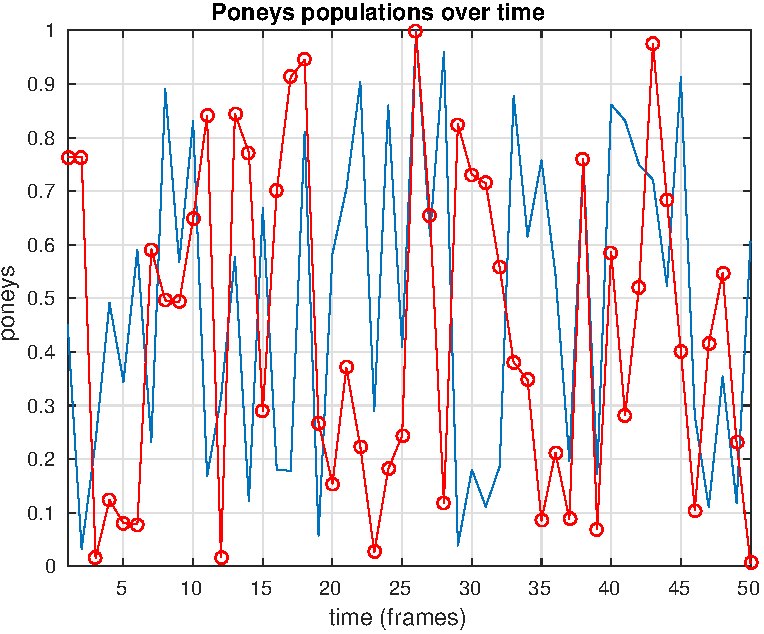
\includegraphics[width=0.5\textwidth]{basicplot.pdf}
  \caption{Basic plot}\label{fig:basic}
\end{figure}


Below are summarised the steps you will have to complete to produce the final graph.
Remember, you can (and \emph{should}) look at the documentation of the functions we will mention.
After completing each step, run your function (typing \mcode{testPlot} in the command line) to see your progress and check for errors.
\begin{enumerate}
  \item Use the \mcode{clf} command to clear the current figure (if present) or open a new empty figure window (1 new line).
  \item Add a line that uses the \mcode{plot} function to display \mcode{R1} with the default settings (1 new line). Then run your code using
  \mcode{testPlot(100)}, to plot 100 random numbers.
  \item Confirm that changing the value of the input argument changes the plot as expected.
  \item \mcode{plot} can take a \textbf{string} input defining the type of the line.
    Look for \emph{LineSpec} information in \mcode{plot} documentation and/or look at the provided examples in the documentation.
  \item Modify your plot line to display \mcode{R1} with a red line.
  \item Modify your plot line to display \mcode{R1} with red open circles joined by red lines.
  \item Try to display \mcode{R2} on the same graph with a new \mcode{plot} call. (1 new line)\\
    By default, MATLAB wipes the previous graph if you call \mcode{plot} twice on the same figure.
    To deactivate this behaviour, you need to use \mcode{hold on} and \mcode{hold off} before and after
    your second \mcode{plot} call.
    Here is an example, adapt it to your case! (2 new lines)
\begin{lstlisting}
plot(x)  % first graph
hold on
plot(y)  % second graph
hold off
\end{lstlisting}
  \item Add a title to your graph, using the \mcode{title} function. (1 new line)
  \item Add axes names to your graph (whatever you like), using the \mcode{xlabel} and \mcode{ylabel} functions. (2 new lines)
  \item Display a grid on your graph, using the \mcode{grid} function. (1 new line)
  \item Limit the x-axis display to the first 50 points, using the \mcode{xlim} function. (1 new line) What happens for different
  input arguments now?
  \item Be proud of your first graph and \textbf{save} it as a .png file using \emph{File/Save As\dots} menu in the figure window.
\end{enumerate}

\textbf{We will look at your work}: \\
Send this figure and the function file you wrote to ``\verb|student_results@mouse.vision|''.
The e-mail Subject should be ``Basic Plotting'' and you should include your group member names in the body.

\pagebreak
\subsection{Advanced plotting: defining axis properties}

Now we will plot something relevant and important to many people.
You will be plotting Google search volume data for a \emph{mystery} search term.
We're not telling you what the search term is right now.
Create a new function file called ``googleTrends.m'' and type the following into it as you go.
Run it after each line is entered to check for errors.\\

First, you have to download the data that originally came from Google Trends:\\
\verb|>> urlwrite('http://mouse.vision/gt.csv','gt.csv');|\\

The data were saved to disk. So read the data into MATLAB and plot them:\\
\verb|>> gt = textread('gt.csv');|\\
\verb|>> plot(gt)|\\
\verb|>> ylabel('search volume')|\\

Each data point shows the search volume for that week for this particular search term.
Let's add one tick mark per year:\\
\verb|>> set(gca,'XTick',0:52:700)|\\

That was a new command you've not seen before.
We won't explain it now, but it should be fairly obvious what it does.
Let's label the tick marks by year:\\
\verb|>> set(gca,'XTickLabel',2004:2017)|\\

Each year marker is placed at January of that year.
Based on this graph, when did the peak popularity for this search term occur?
Hmmm\ldots so what could this search term be?
Yell out your suggestions \textbf{very loudly}.


\pagebreak
\subsection{Advanced plotting: images and histograms}

You will now try more advanced plots.
The aim is to plot an image and an histogram of some random data.
First, create a new function called \mcode{testImage} in a new file \verb|testImage.m|.
In this function, do the following steps that will lead you to success:
\begin{enumerate}
  \item create a 100-by-100 matrix of random data and store it in a variable \mcode{R} (see \mcode{help rand}),
  \item create a new empty figure window (use the \mcode{clf} function),
  \item display in this figure \mcode{R} as an image (use the \mcode{imagesc} function),
  \item add a title (use the \mcode{title} function),
  \item run your function in the command line and \textbf{save} your figure as a .png image.
\end{enumerate}
You should obtain something similar to Figure~\ref{fig:adv}~(a).

\begin{figure}[h]
  \centering
  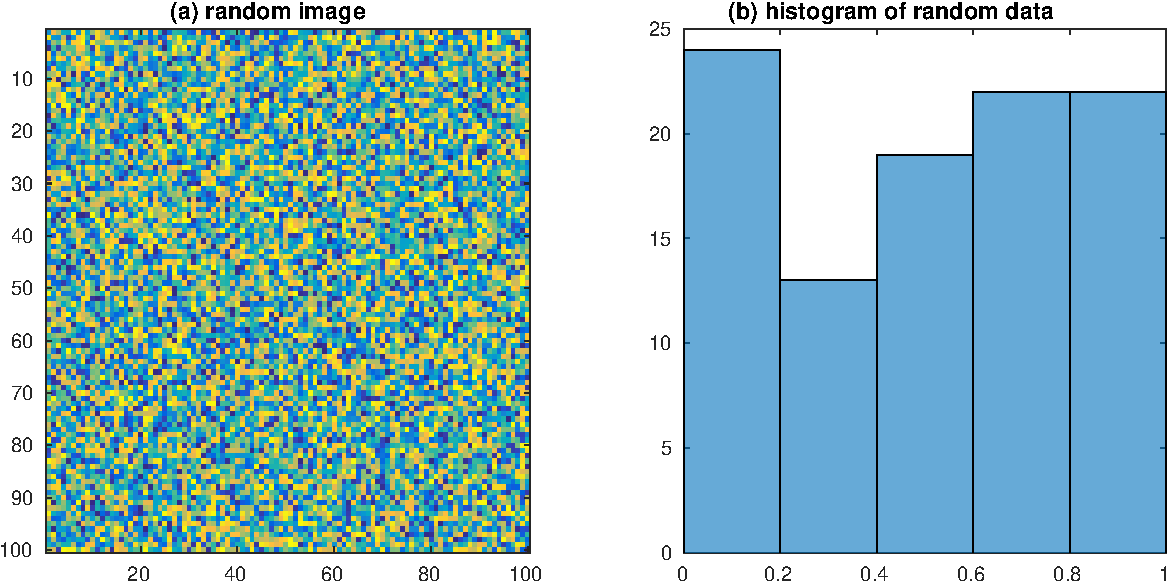
\includegraphics[width=0.7\textwidth]{advancedplot.pdf}
  \caption{Advanced plots: (a) and image or surface plot. (b) a histogram.}\label{fig:adv}
\end{figure}



Now, for the next graph: the histogram! Create a \mcode{testHist} function in a new file \verb|testHist.m|:
\begin{enumerate}
  \item create a vector (one column or one row) of 100 random numbers and store it in a variable \mcode{R},
  \item display the histogram of \mcode{R} on this figure (use \mcode{hist} or \mcode{histogram}),
  \item run your function in the command line and \textbf{save} your figure as a .png image.
\end{enumerate}
You should obtain something similar to Figure~\ref{fig:adv}~(b).
If that was too easy for you and you want a challenge, try making the histogram bars red and increasing the number of bins in the histogram.
Otherwise, proceed to the next section.

\textbf{We will look at your work}: \\
Send these figures and the function files you wrote to ``\verb|student_results@mouse.vision|''.
Ensure the Subject is ``Advanced Plotting'' and that you include your group member names in the body.

\pagebreak

\section{Conditional expressions with \emph{if\dots else} statement}

\textbf{Conditional expressions} are really important since they allow you to add logic to a function.
In other words, conditional expressions allow you to make certain events happen only under certain conditions.
For example, you could use a conditional expression to make a plot only if a vector is longer than a certain length.

Let's get started by looking at \mcode{if} statements.
The conditional expression starts with the \mcode{if} keyword, followed by the condition, then the code to be executed if the condition is true, and finally the \mcode{end} keyword to close the expression.
Type the following in a new function called \mcode{testIf.m}
\begin{lstlisting}
function testIf(a)
  if a < 10
    disp('a is less than 10')
  elseif a > 10
  	disp('a is greater than 10')
  end
  disp('this always runs')
\end{lstlisting}

Now run your code using \mcode{testIf(2)} (this makes the variable \mcode{a} take on the value 2).
What happens? \\
What happens if you run your function with the input being \mcode{42}?\\
What happens if you run your function with the input being \mcode{10}?\\
Can you make the function report when the input is \mcode{10}? Hint: the \mcode{else} keyword.

You have now learned the basics of logic statements!

\pagebreak


\section{Repeating operations with \emph{for} loops}

Let's run the previous function, \mcode{testIf}, many times in an automated way.
First of all, remove the final \mcode{disp} command in \mcode{testIf} and re-save the function file.
Now create a new function called \mcode{testForLoop} and type the following into it:

\begin{lstlisting}
function testForLoop(N)
  % loop from 1 to N times
  for ii=1:N
    disp(ii)  % display current value of ii
    testIf(ii)
  end

\end{lstlisting}

Run it with \mcode{N} being 20. What happens? Now try N being 5.

As you can see, the \textbf{for} loop starts with the \mcode{for} keyword, followed by the increment expression (e.g. \mcode{ii=1:10}), then the code for what happens in each pass through the loop and finally the \mcode{end} keyword to close the loop definition.
At each iteration, the loop variable (\mcode{ii} in the above example loop) gets the next value from the vector defined on the right of the \mcode{=} (equal) symbol. If this is confusing, please ask for help.

Complete the following function to make it multiply each element of the variable \mcode{R1} by N:
\begin{lstlisting}
function multiplyLoop(N)
  % exercise function

  R1 = rand(1,12);  % initialize R1 with random values
  disp(R1);         % display initial contents of R1

  % HERE, YES RIGHT HERE, YOU SHOULD PUT A LOOP.

  disp(R1)          % display updated R1
\end{lstlisting}

In general, even if loops are great, you can do the same operations more efficiently using array indexing and functions.
Add a line at the end of the function that multiplies \mcode{R1} by \mcode{N} without using a loop (using only the arithmetic operators you learned at the start).


\textbf{We will look at your work}: \\
Send the function file you wrote to ``\verb|student_results@mouse.vision|''.
Ensure the Subject is ``For Loops'' and that you include your group member names in the body.


\pagebreak
\section{(Bonus) More exercises}

If the above was easy and you finished quickly, try the following exercises.
Each of these should be done in a separate function file.

\begin{enumerate}

\item Use \mcode{rand}, \mcode{round}, and \mcode{*} to produce a vector of 5000 random integers having values between 0 and 20.
Use the \mcode{unique} command to confirm that you have values from 0 to 20 and no others.
Use the \mcode{hist} command to make a histogram of the distribution.
Plot the histogram with 21 bins, since you have that many unique numbers.
Does it look like a uniform distribution? Replace \mcode{round} with \mcode{ceil} and repeat.
Is it uniform now?

\item Using the random vector you generated in the previous exercise, apply the \mcode{find} command and the \mcode{length} command to count the number of times the number 10 occurred.
  Does this number match what the histogram showed?

\item Repeat the previous exercise (ignoring the histogram) and count how many times a number less than or equal to two occurred.
  Repeat again and count the number of times a number less than or equal to three occurred.
  Now write a \mcode{for} loop that performs this count for all numbers between 1 and 20 (which are the unique numbers in the vector).

\item Build a 9 by 10 array. Plot this in an array of 3 by 3 subplots.
  Each subplot contains data from one row of the matrix (hint: array indexing).
  Waveforms should be red lines with no symbols.
  Add a green circle at the maximum value of each plot (hint: help max).

\end{enumerate}

\section{Additional resources}

You want more?
Right, here are some nice online resources to complete and go beyond this tutorial:
\begin{itemize}
  \item the MIT MATLAB course,\footnote{%
    \url{http://ocw.mit.edu/courses/electrical-engineering-and-computer-science/6-094-introduction-to-matlab-january-iap-2010/}
  }
  \item tutorialspoint.com course,\footnote{%
    \url{http://www.tutorialspoint.com/matlab}
  }
  \item Software Carpentry tutorial.\footnote{%
    \url{http://swcarpentry.github.io/matlab-novice-inflammation/}
  }
\end{itemize}

The last website, Software Carpentry, is a goldmine for data analysis.
Check their lessons\footnote{\url{http://software-carpentry.org}} if you want to learn more about other tools and programming languages used to crunch data.

Happy analysis!

\end{document}
